%!TEX root=../ctl-phd-thesis.tex

\section{Supplementary Information}
\subsection{Application of the Bayesian scheme to MD}
  \par To infer from the trajectory the intrinsic system force and the diffusivity, the latter are represented by cubic interpolants, which admit a continuous first derivative. These interpolants are evaluated at equally spaced values, $z_i$, of the transition coordinate. Under these premises, the position-dependent diffusivity writes,
%
\begin{equation}
D(z) = a_i^{(0)} + a_i^{(1)} \left(\frac{z-z_i}{h}\right) + a_i^{(2)} \left(\frac{z-z_i}{h}\right)^2 + a_i^{(3)} \left(\frac{z-z_i}{h}\right)^3
\end{equation}
%
  where $a_i^{(0)}$, $a_i^{(1)}$, $a_i^{(2)}$ and $a_i^{(3)}$ are functions of $a_{i-1}$, $a_i$, $a_{i+1}$ and $a_{i+2}$, that is a set of parameters $\{ a_i \}$. The intrinsic system force, which depends on $z$, can be expressed in a similar fashion, as a function of a set of parameters $\{ b_i \}$. The probability $P[(z_{k+1}, t_{k+1} | z_k, t_k) | F(z,t), D(z)]$ can be interpreted as the likelihood of observing the transition from $z_k$ at time $t_k$ to $z_{k+1}$ at time $t_{k+1}$ under the action of a time-dependent bias, $F_{{\rm bias}, k}$, given the sets of parameters $\{ a_i \}$ and $\{ b_i \}$. $z_k$ and $F_{{\rm bias}, k}$ are data readily available from the trajectory. By virtue of Bayes' theorem, the posterior probability of the parameters $\{ a_i \}$ and $\{ b_i \}$, given $z_k$ and $F_{{\rm bias}, k}$, can be expressed as,
%
\begin{equation}
\label{Bayes}
P(\{ a_i \}, \{ b_i \} | z_k, F_{{\rm bias}, k}) =
P(z_k, F_{{\rm bias}, k} | \{ a_i \}, \{ b_i \}) \times P_{\rm prior}(\{ a_i \}, \{ b_i \})
\end{equation}
%
  \par The prior probability, $P_{\rm prior}(\{ a_i \}, \{ b_i \})$, of the sought parameters can be of different nature --- it embraces a number contributions ensuring that $\{ a_i \}$ be scale invariant, that the intrinsic system force obtained from $\{ b_i \}$ do not depart significantly from that measured in the biased simulation, and that $D(z)$ be smooth over an appreciable length scale.

  \par The diffusivity and the intrinsic system force --- or the potential of mean force, are subsequently determined by means of a Metropolis-Hastings algorithm, which generates a Markovian chain of states characterized by consecutive values of the parameters $\{ a_i \}$ and $\{ b_i \}$. We refer the reader to reference \citenum{Comer2013} for the computational details of the algorithm.

\subsection{Qualitative Analysis}

\par In some of the MD trajectory snapshots, we observed conditions in accord with that of others. Shown in Fig \ref{fig:cod_bowed}, is the distortion of the bilayer when codeine is constrained at some distance away from the bilayer. Similarly, in Fig \ref{fig:waterfinger}, is shown water molecules traversing the bilayer to solubilize the charged urea, a result previously also described by Cardenas et al\cite{Cardenas2012}. In an attempt to quantify the prevalence of membrane deformation and water finger patterns, an MDAnalysis script\cite{Michaud-Agrawal2011} was used to bin the positions of phosphates and waters (\textit{i.e.,} those within 5~\AA\, in the $x$ and $y$ directions). The probability distributions for several time blocks from US urea are shown in Fig.~\ref{fig:distributions}. The choice of phosphate atoms as the reference defining bilayer normal is not optimal due to the substantial rearrangement of phospholipids. Due to the small membrane size, the asymmetry induced by the crossing permeant on headgroup locations will lead to a moving center of membrane reference influencing results.

\begin{figure}[htbp]
\begin{center}
	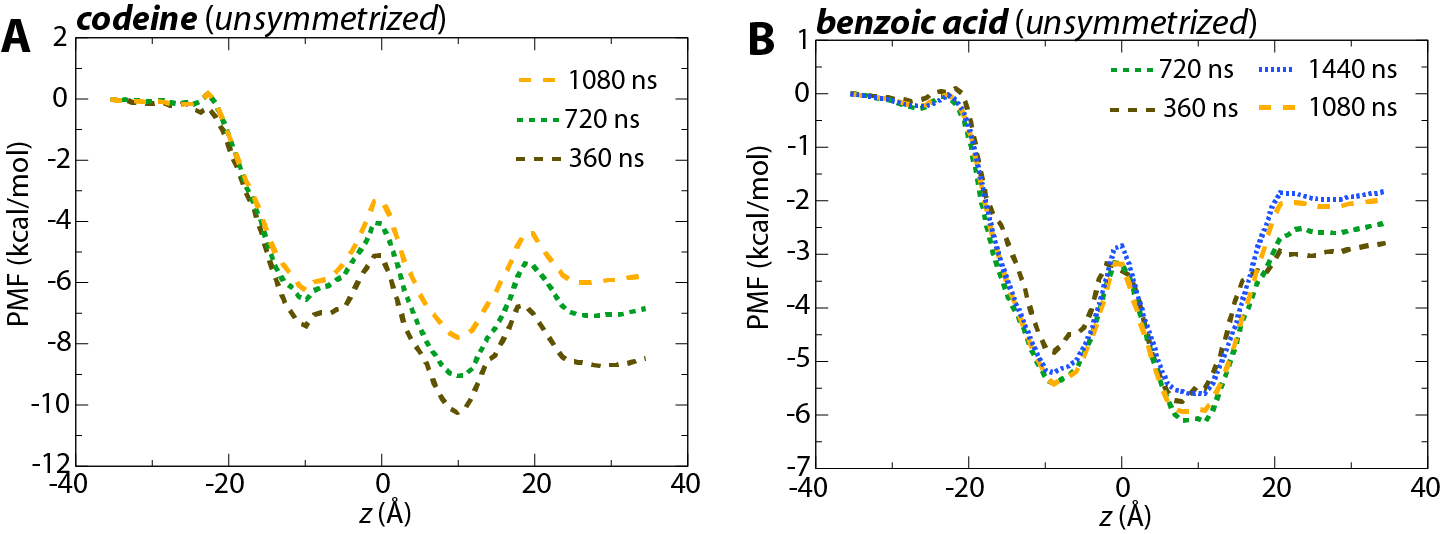
\includegraphics[width=1.0\textwidth]{Figures/asym-codbenz}
	\caption[Unsymmetrized PMFs for codeine and benzoic acid from REUS]{Unsymmetrized PMFs for (A) codeine and (B) benzoic acid from REUS.
	}
	\label{fig:asym-others}
\end{center}
\end{figure}

\begin{figure}[htbp]
\begin{center}
	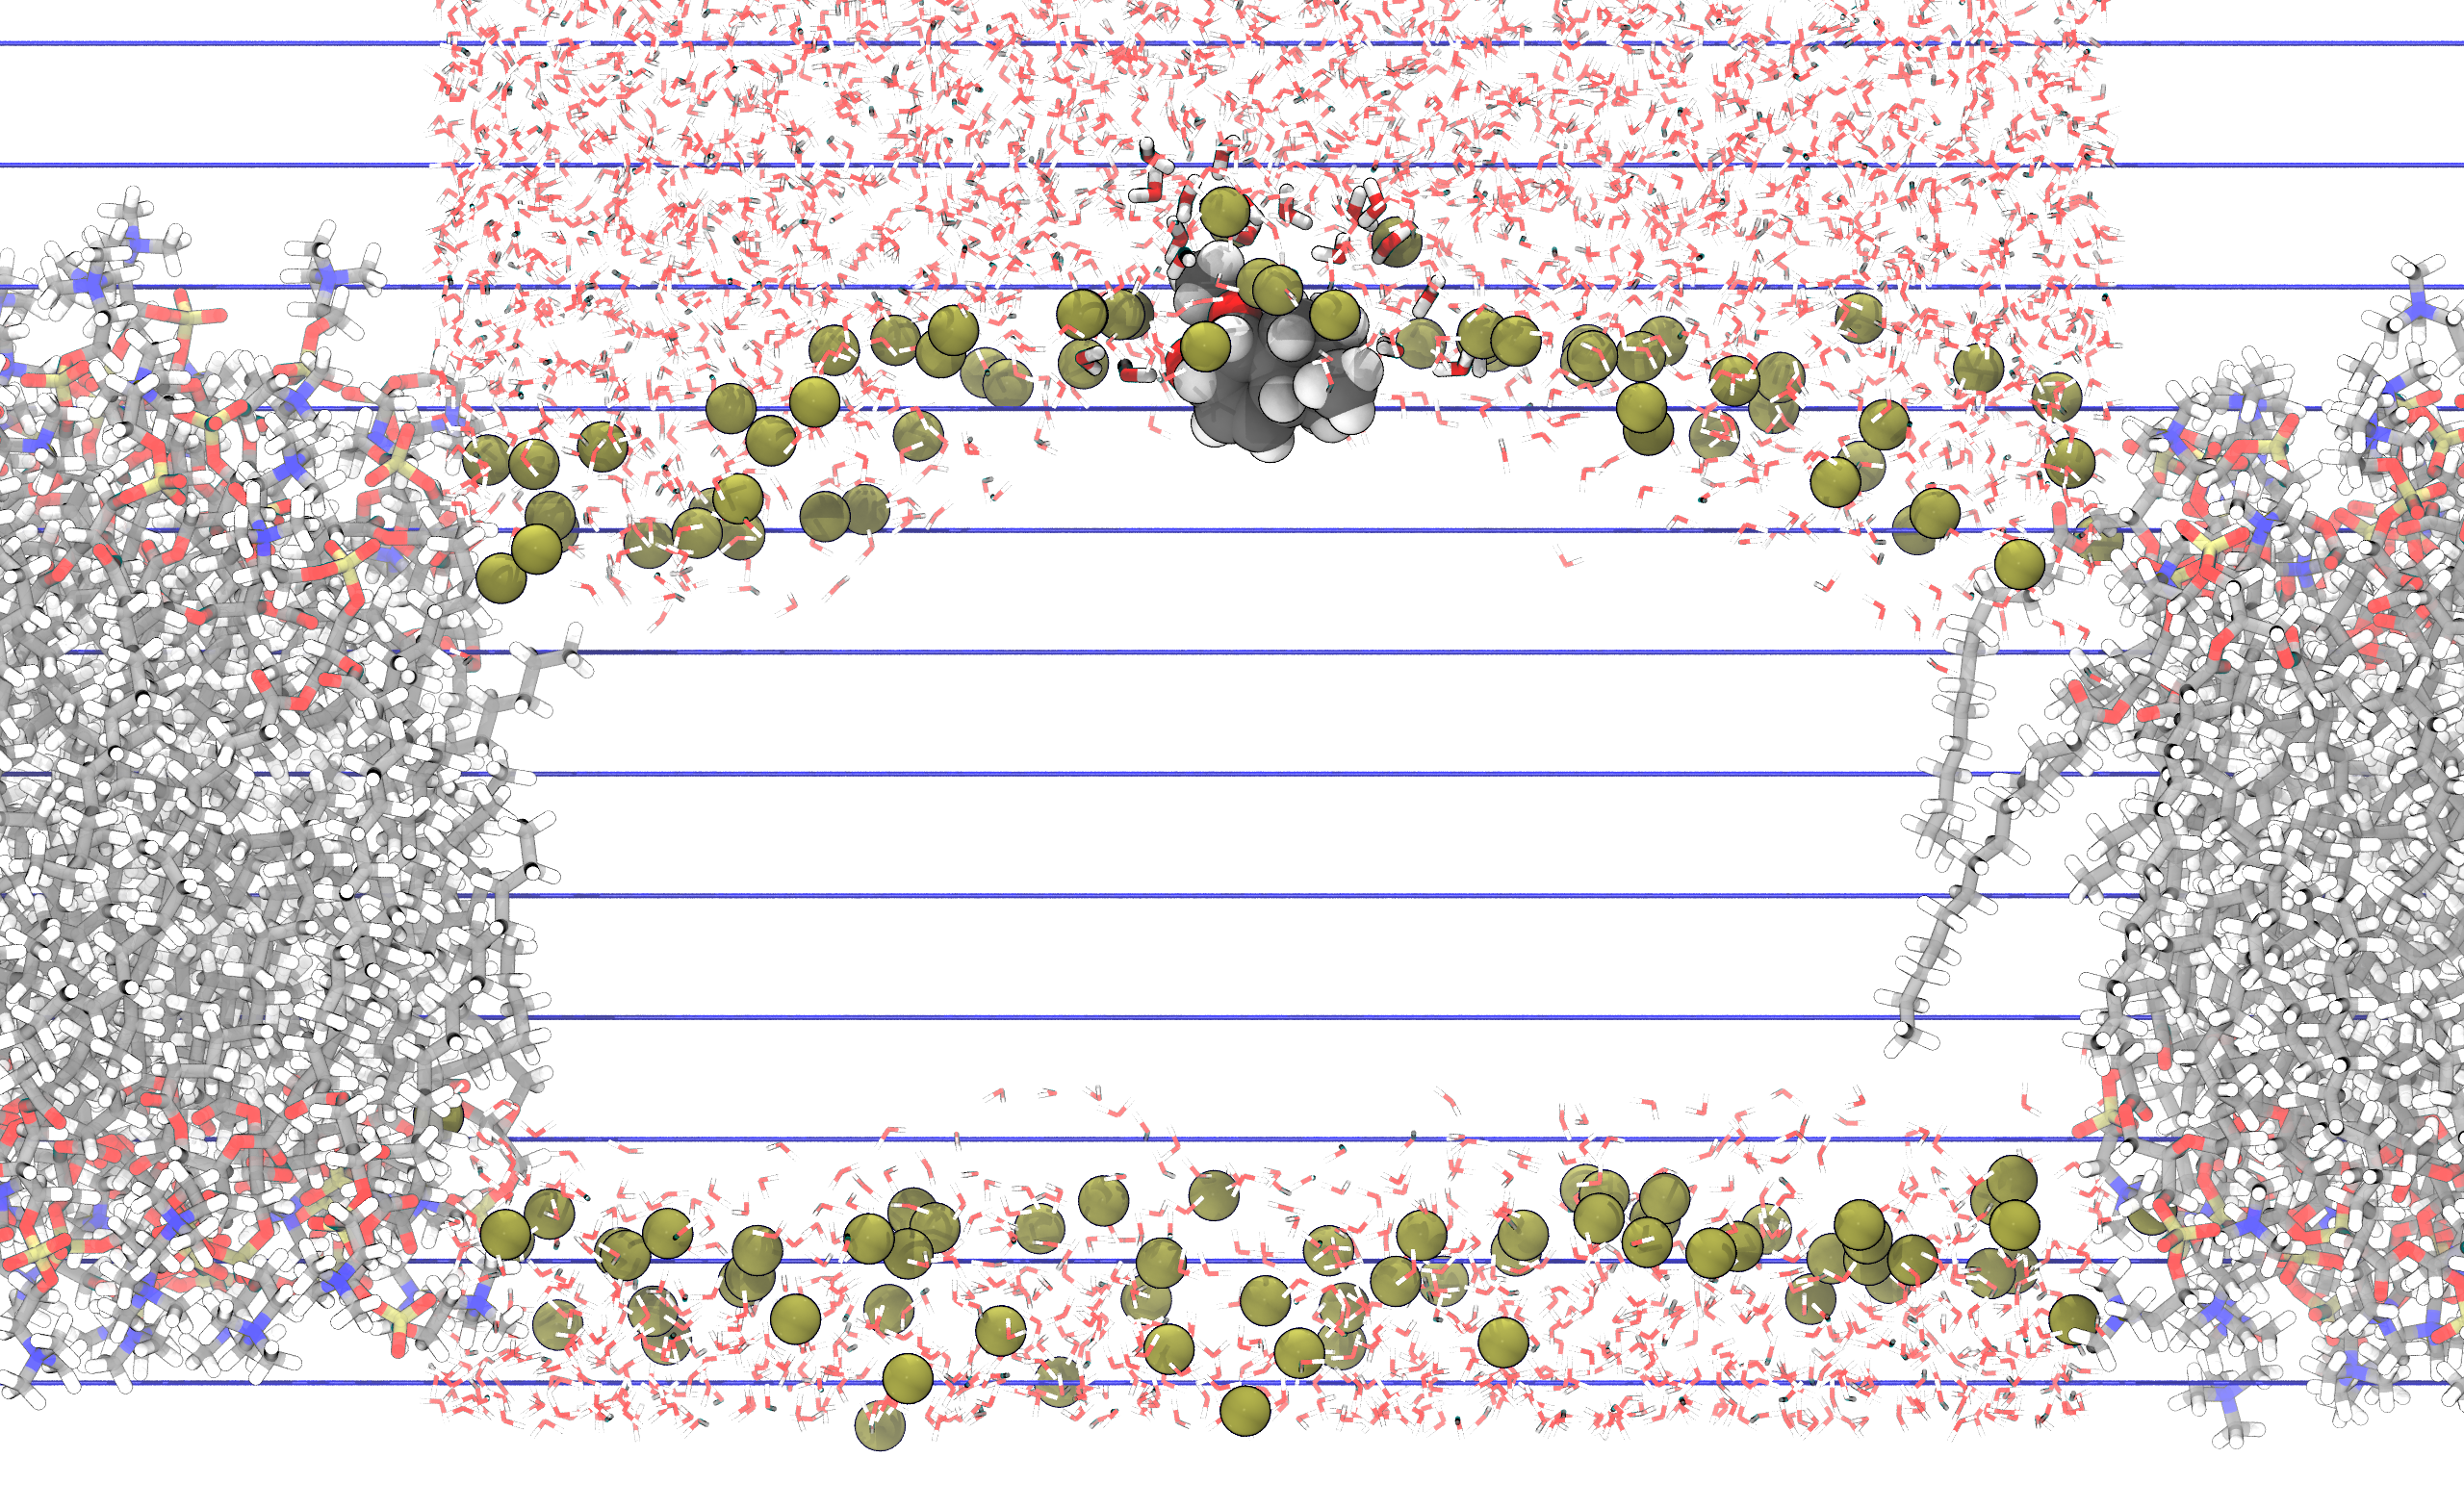
\includegraphics[width=0.8\textwidth]{Figures/cod_bowedmembrane}
	\caption[Illustration of harmonically constrained codeine bowing the membrane to interact with hydrophobic lipid tails]{A VMD rendered snapshot from the US of codeine constrained at $z=-20$.
	The lipids in center have been hidden, and lateral periodic images shown. Phosphates are shown as yellow spheres illustrating the bowing of the top leaflet to solubilize the hydrophobic rings. Water molecules within 5~\AA\ of codeine are shown as licorice, while all other waters are lines.}
	\label{fig:cod_bowed}
\end{center}
\end{figure}

\begin{figure}[htbp]
\begin{center}
	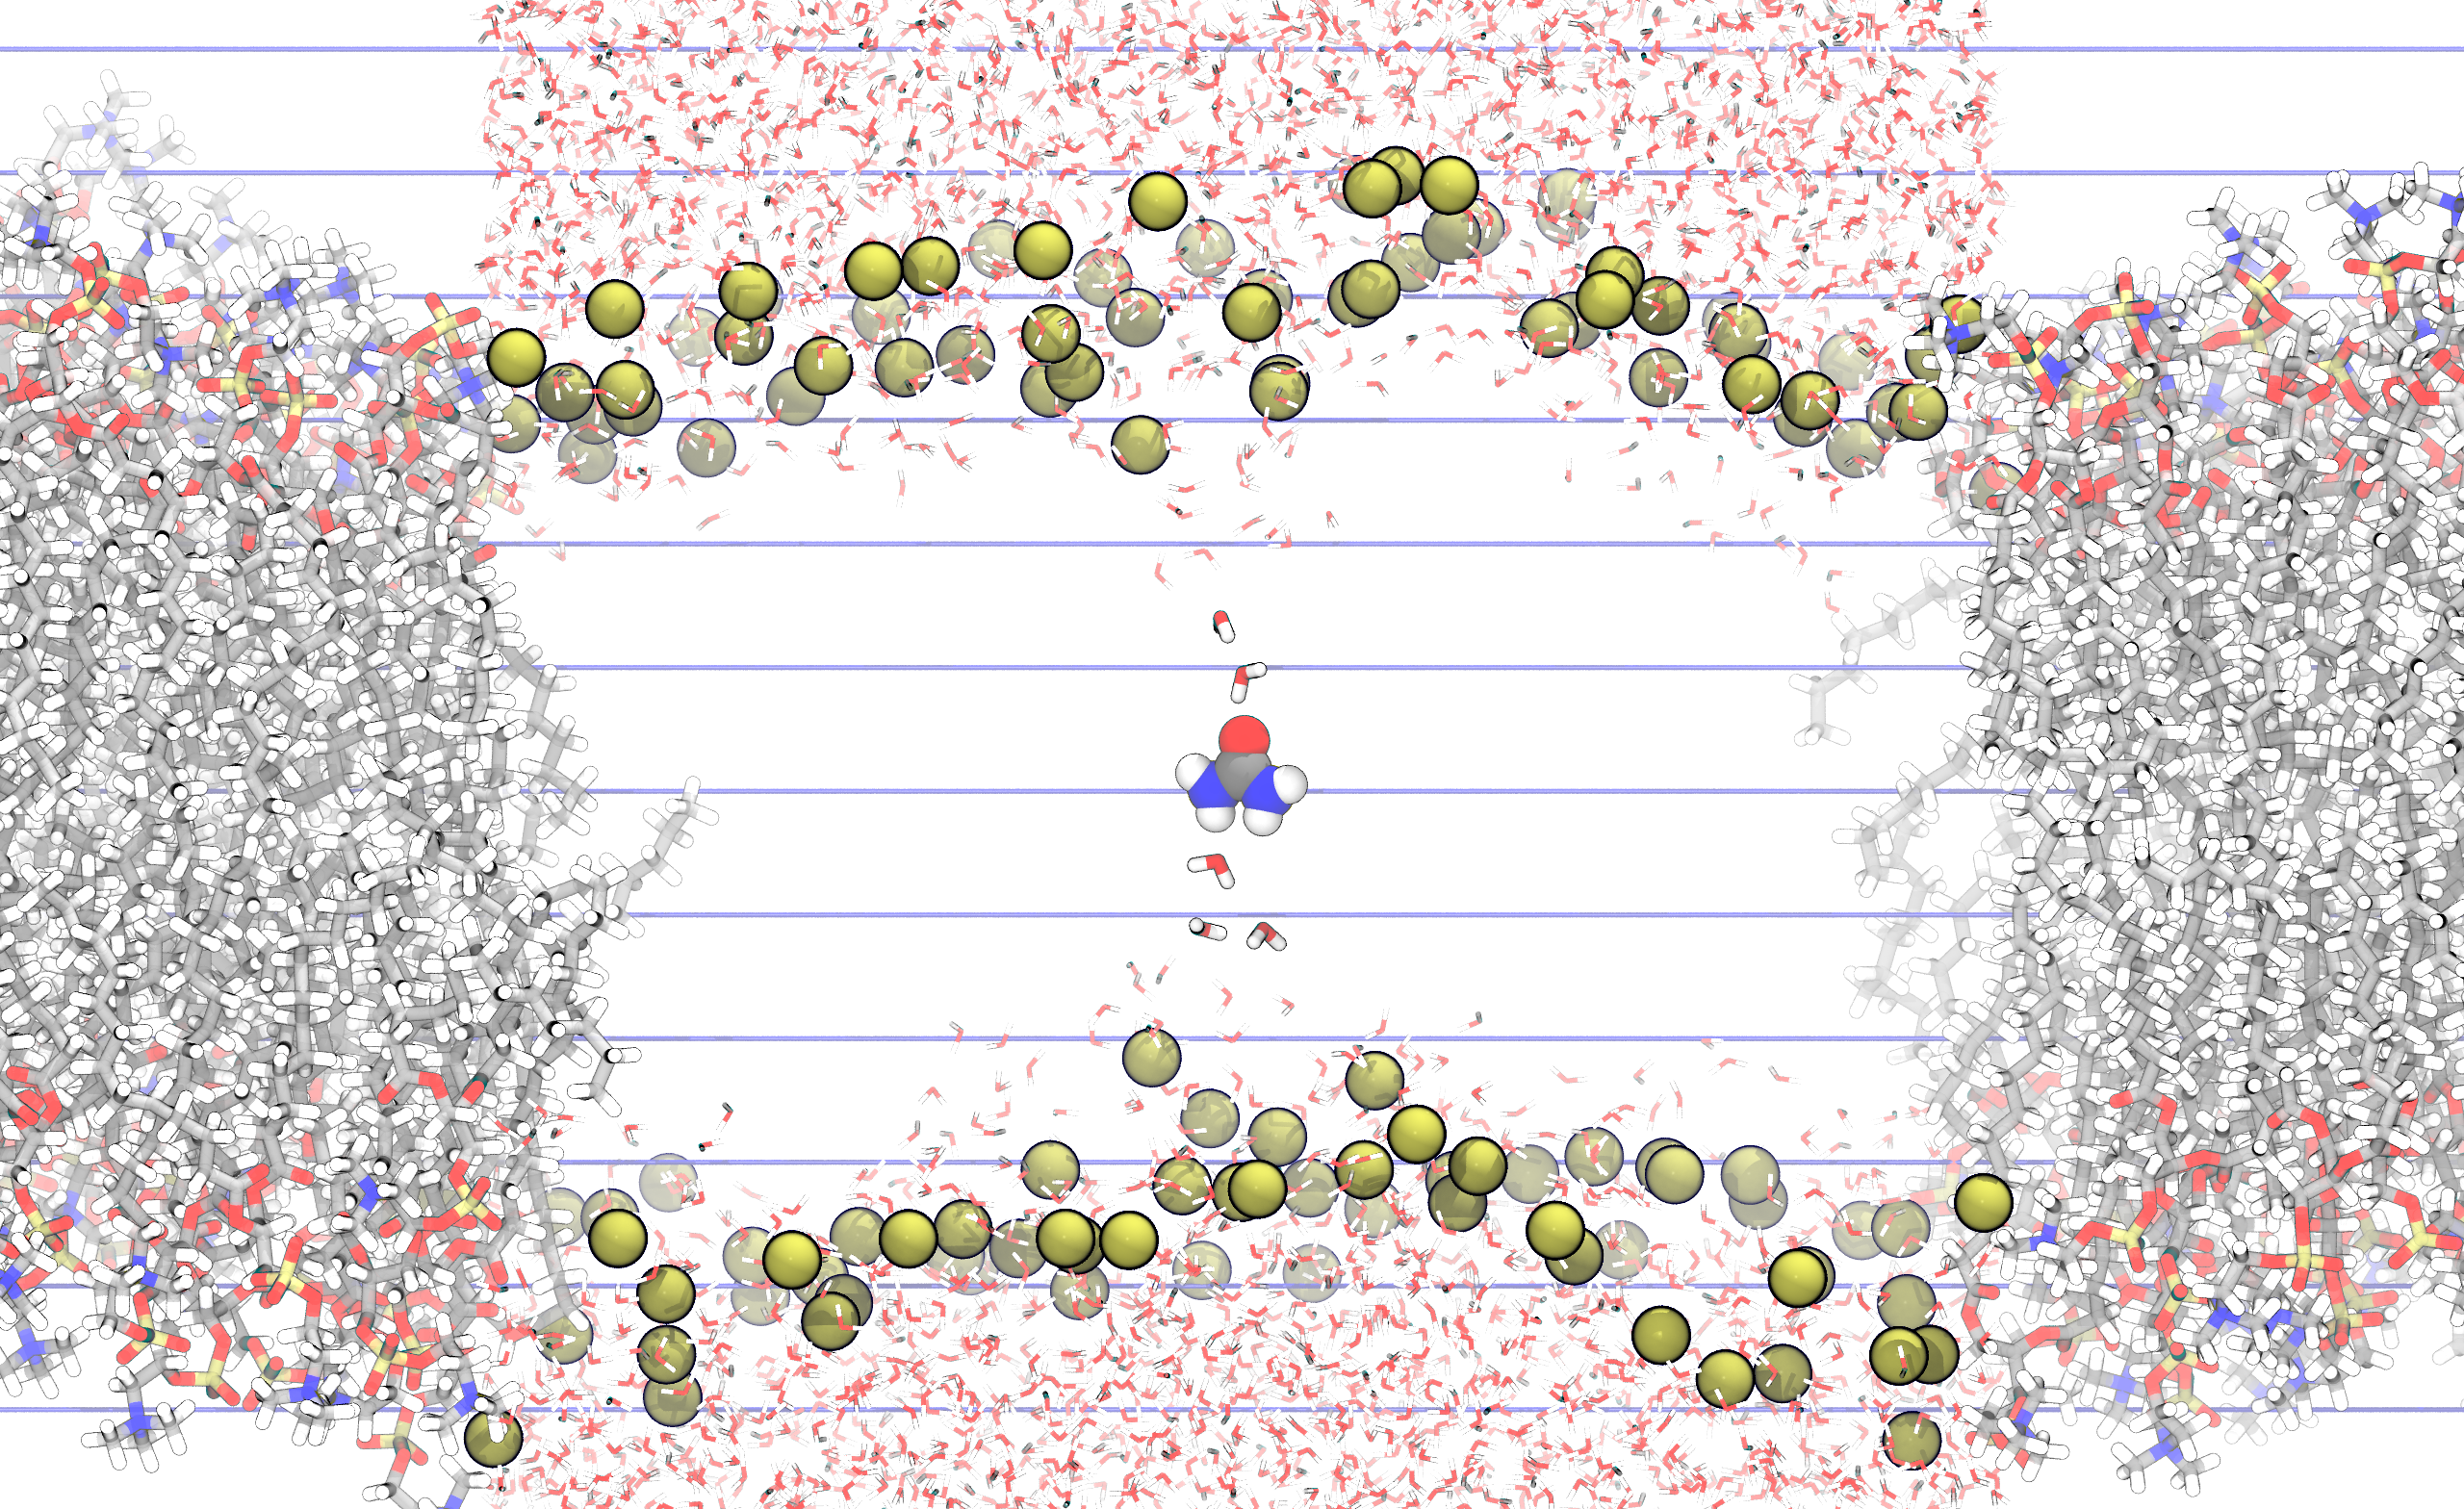
\includegraphics[width=0.8\textwidth]{Figures/urea_waterfinger}
	\caption[Illustration of harmonically constrained urea forming water fingers across the bilayer]{A VMD rendered snapshot from the US of urea constrained at $z=0$. The lipids in center have been hidden, and lateral periodic images shown. Phosphates are shown as yellow spheres. Water molecules within~5\AA\ of urea are shown as licorice.}
	\label{fig:waterfinger}
\end{center}
\end{figure}

\begin{figure}[htbp]
\begin{center}
	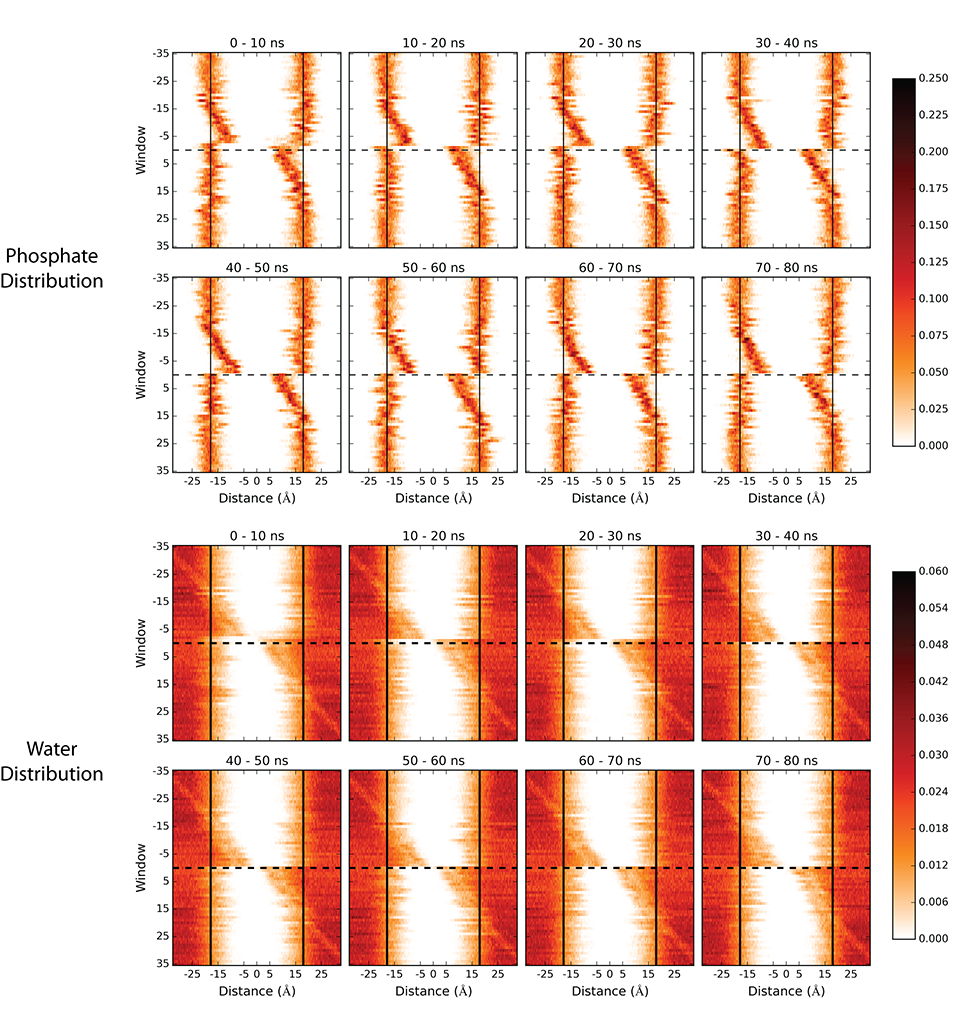
\includegraphics[width=0.9\textwidth]{Figures/distributions1}
	\caption[Probability distributions of phosphate headgroups and water molecules from umbrella sampling calculations]{The normalized probability density of phosphates and water molecules within $5$~\AA\, in the $x$ and $y$ dimensions of urea are shown as a heatmap. The window reflects the $z$-value reference of the US harmonic constraint. A dotted line is placed at window $z=0$ for visual reference. Residual non-equilibrium effects can be seen as deviations of the membrane divot from $z=0$. It appears that both phosphate and water distributions approach the middle after ~30 ns of sampling. The vertical black lines highlight the DMPC average phosphate position at equilibrium without permeant. Note the diagonal observed from the upper left to bottom right of the water distribution is not an artifact. The constrained permeant occupies this position and displaces some waters.}
	\label{fig:distributions}
\end{center}
\end{figure}

\begin{figure}[htbp]
\begin{center}
	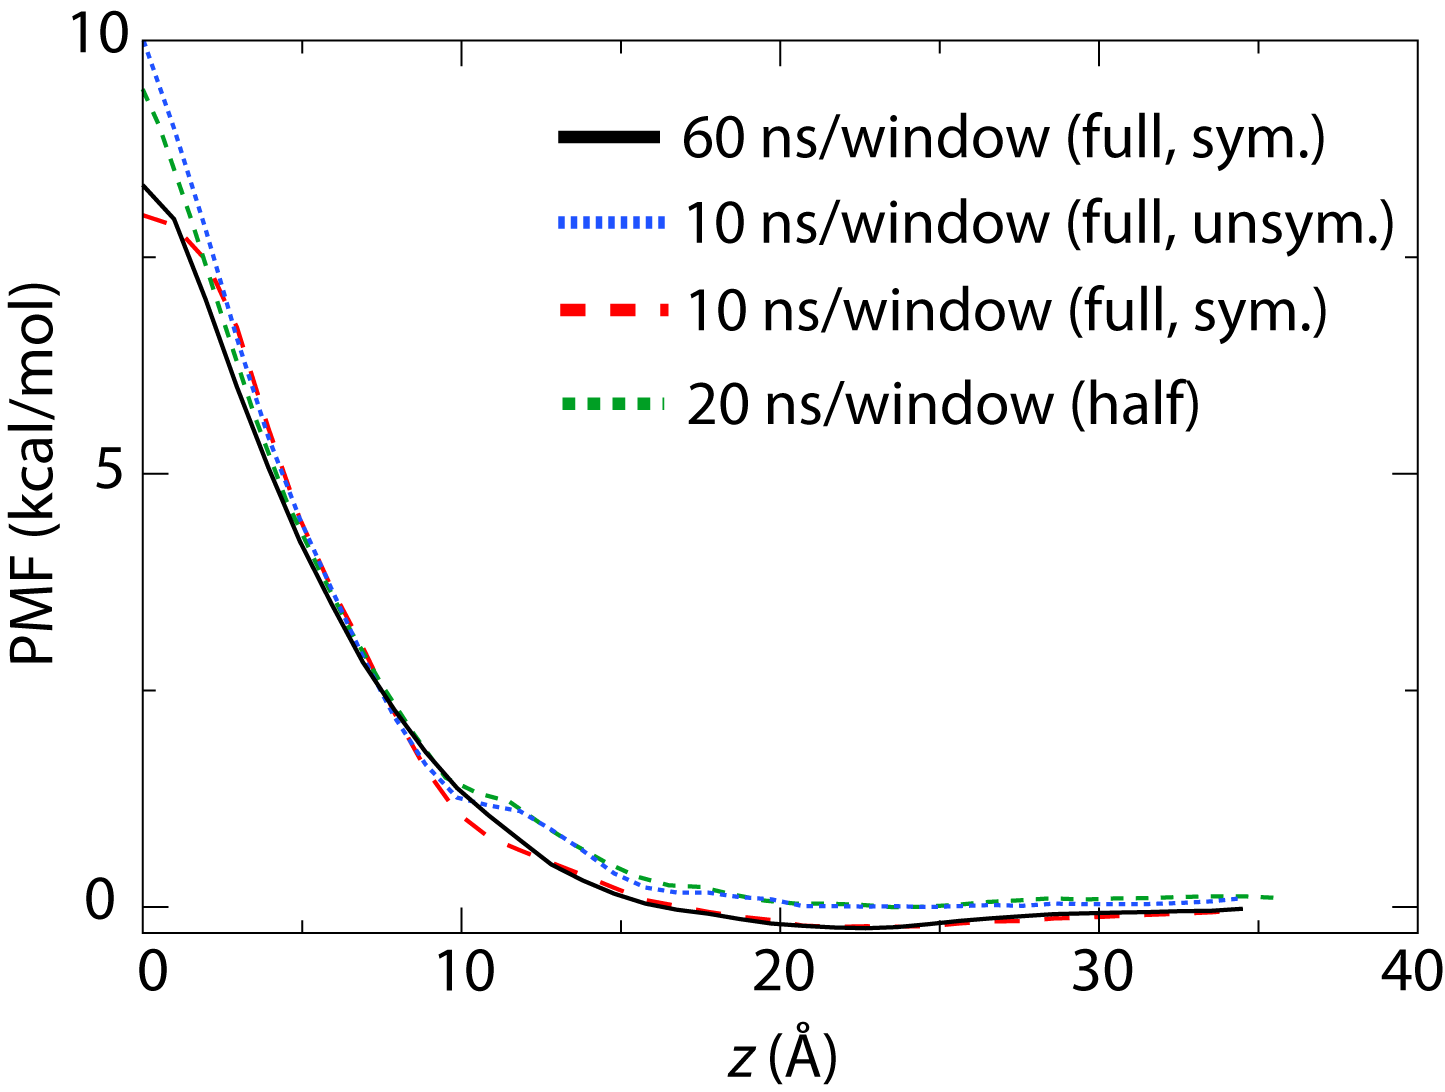
\includegraphics[width=0.8\textwidth]{Figures/compare-half}
	\caption[Comparison of PMFs calculated using REUS using symmetrized half bilayer or full bilayer]{PMFs for urea calculated using REUS.  The PMFs are shown for only the range $z$=(0,36).  The term ``full'' represents that the REUS calculation was performed for 72 windows spanning the entire bilayer, whereas ``half'' means only 36 windows spanning the range from the bulk to the membrane center were used. ``sym.'' or ``unsym.'' refers to whether or not the PMFs for the full range were symmetrized.}
	\label{fig:comparehalf}
\end{center}
\end{figure}


\begin{figure}[htbp]
\begin{center}
	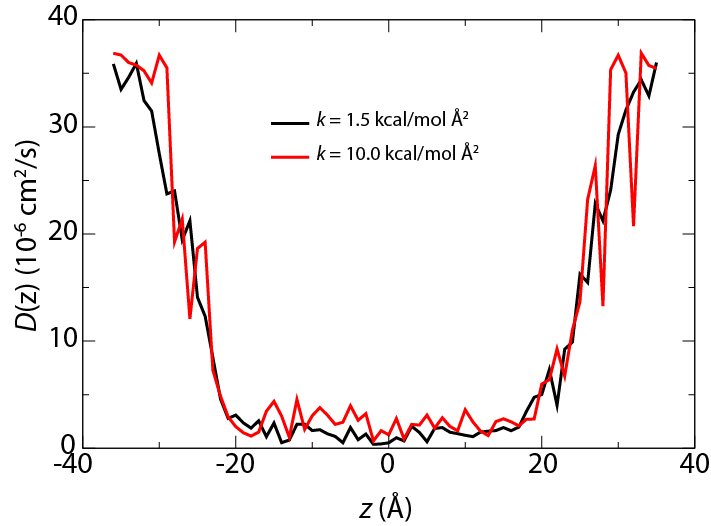
\includegraphics[width=0.8\textwidth]{Figures/D-k10-k1-5.png}
	\caption[Diffusivity profiles for urea calculated using the Generalized Langevin method with different force constants]{Diffusivity profiles for urea calculated using the Generalized Langevin method with different force constants.  The black line is for $k=1.5$~kcal/mol$\cdot$\AA$^2$, calculated from 1-\AA-spaced windows run for 10-ns each, i.e., those also used for the PMF calculation.  The red line was computed from 2-ns simulations in each window with a force constant $k=10$~kcal/mol$\cdot$\AA$^2$.}
	\label{fig:compareK}
\end{center}
\end{figure}

\begin{figure}[htbp]
\begin{center}
	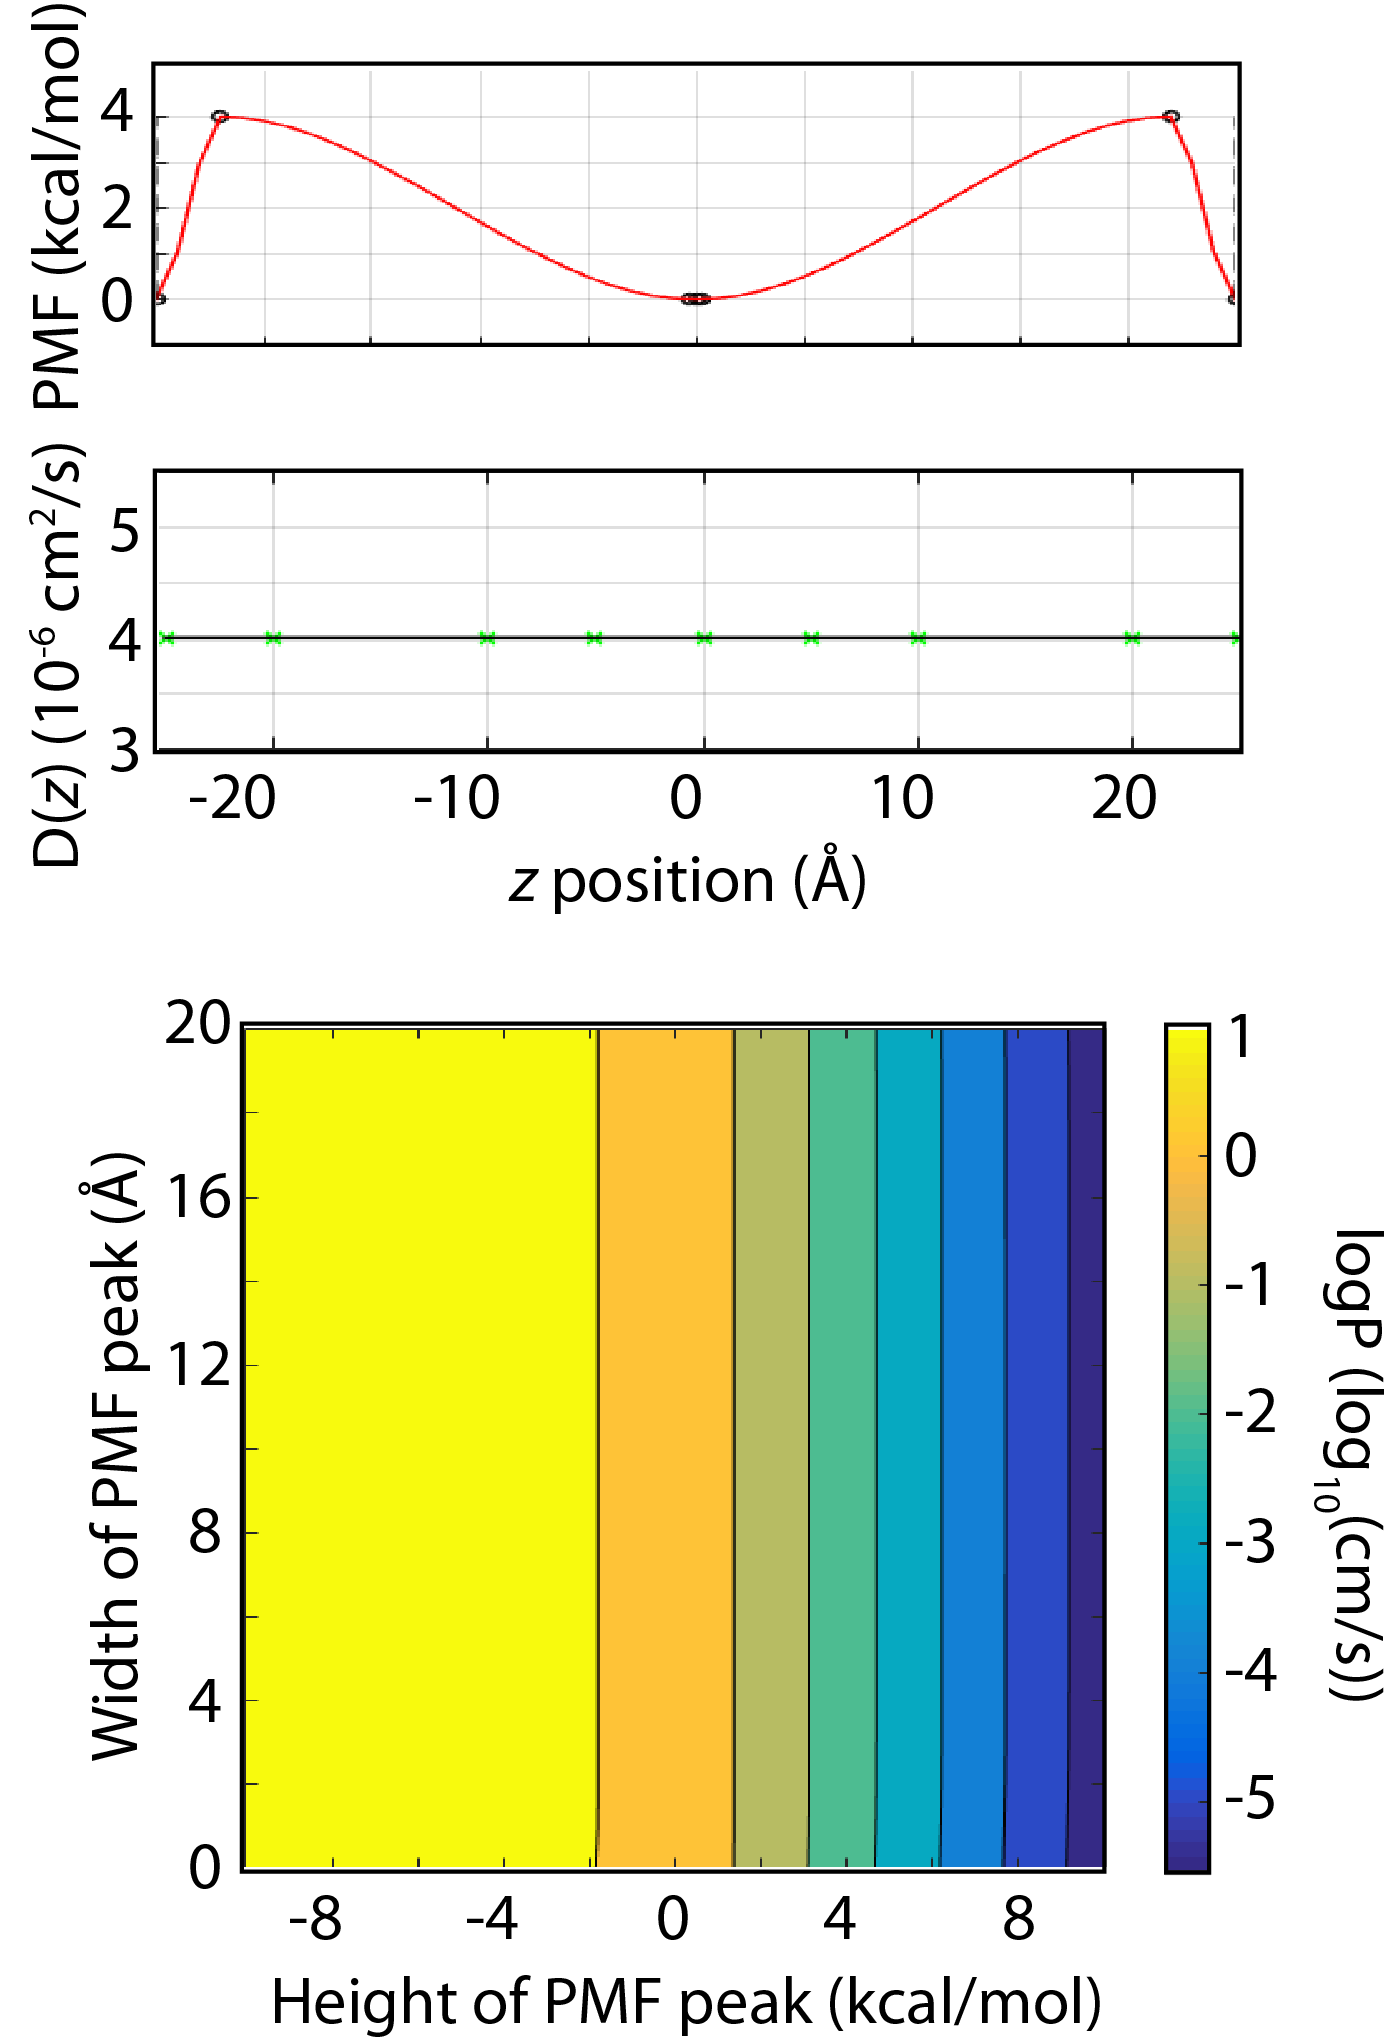
\includegraphics[width=0.8\textwidth]{Figures/SFig-W1}
	\caption[LogP$_m$ as a function of modeled input]{LogP$_m$ as a function of modeled input. The input PMF and $D$($z$) are shown on top and the dependence of logP$_m$ on bottom.  The height and width of the two peaks in the PMF at the membrane-water interfaces are varied while $D$($z$) is held constant. }
	\label{fig:models2}
\end{center}
\end{figure}

\begin{figure}[htbp]
\begin{center}
	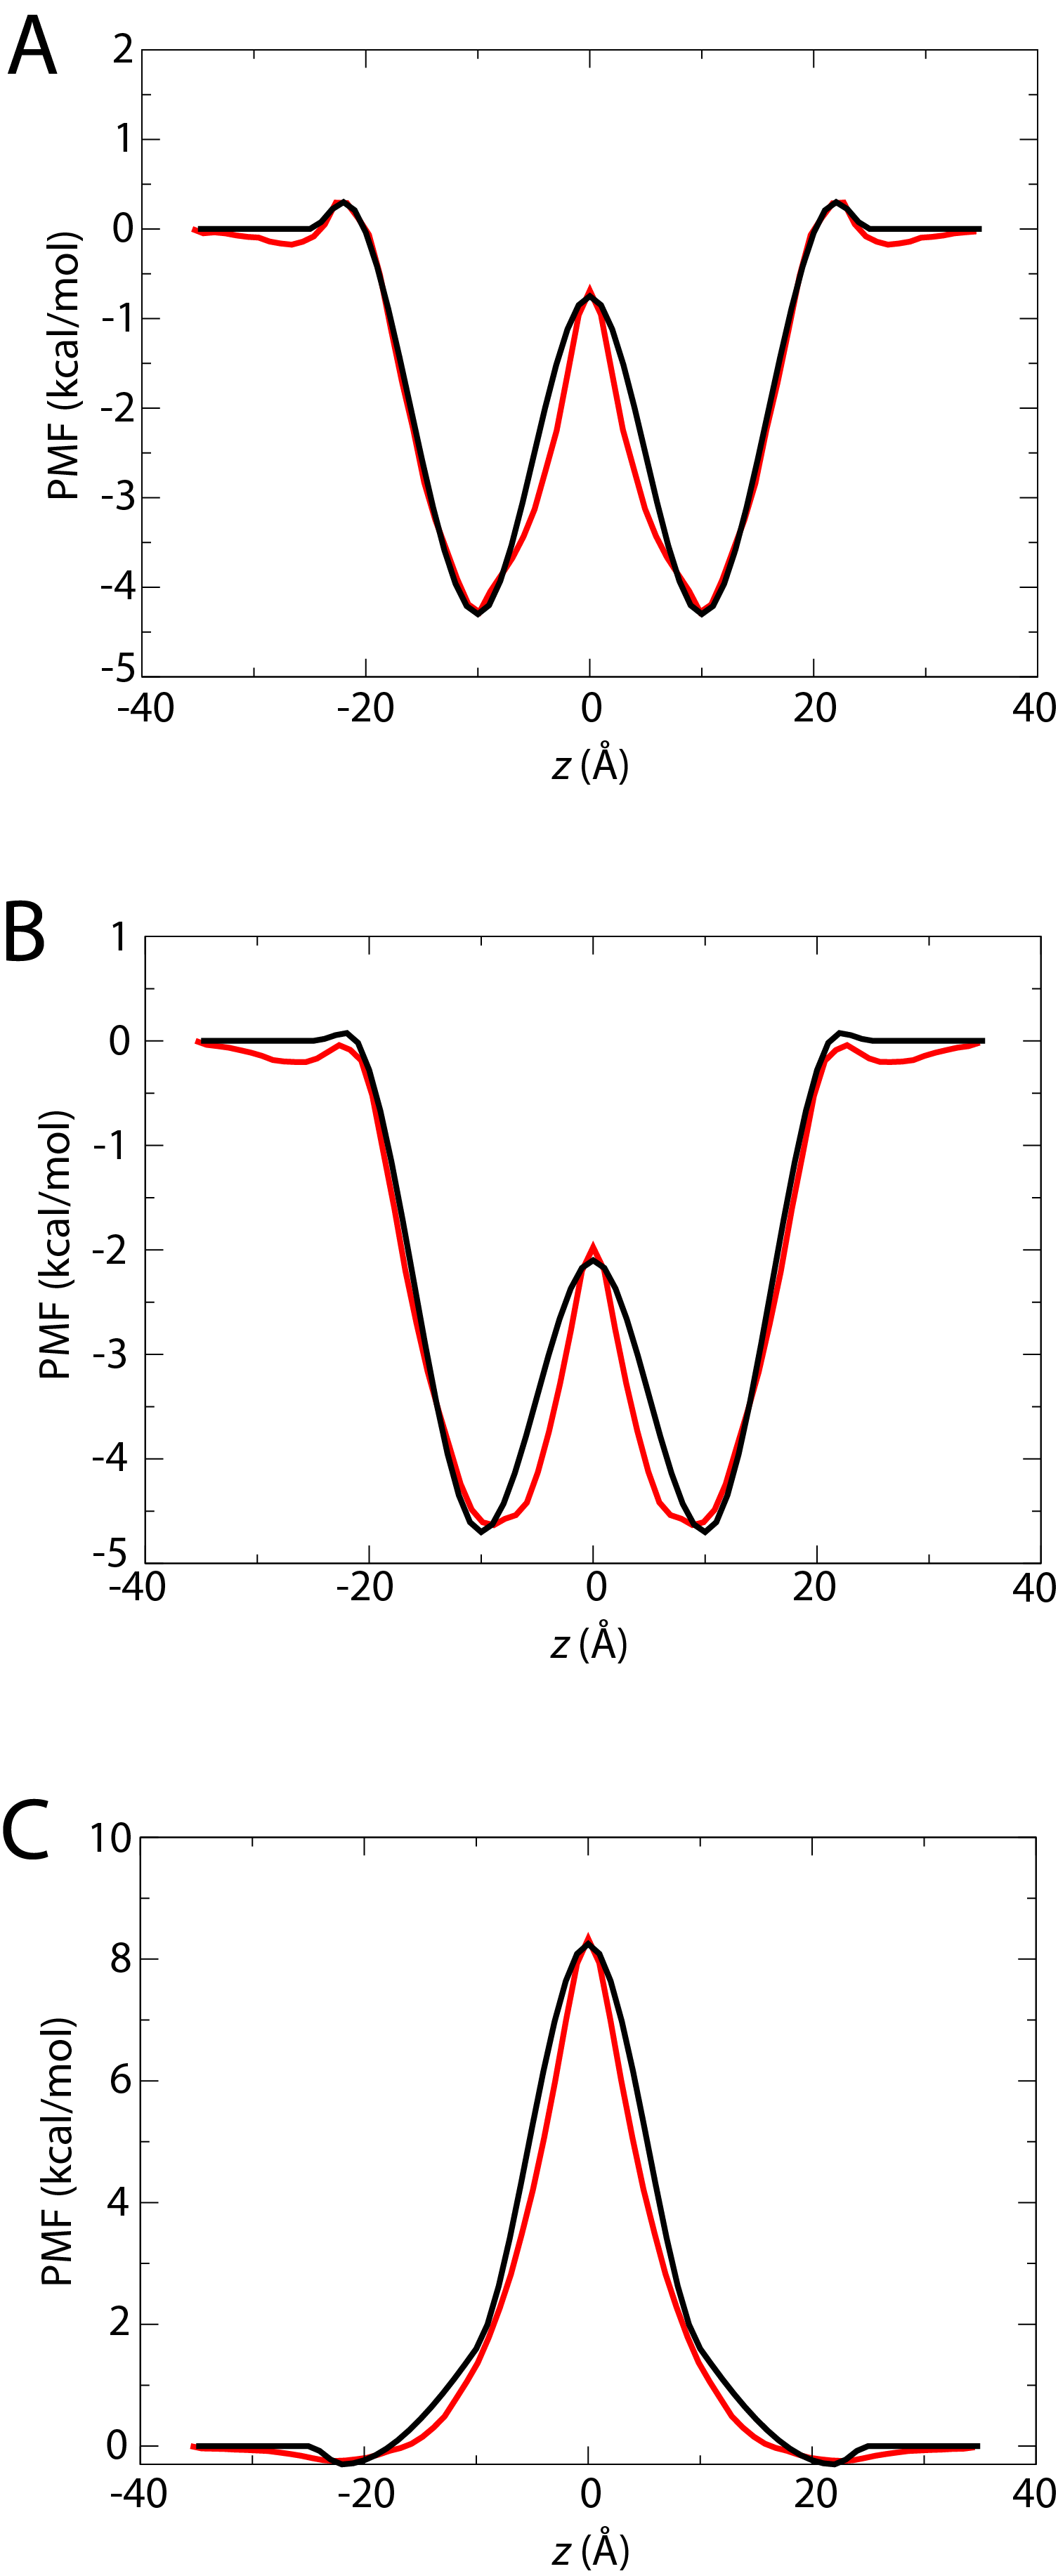
\includegraphics[width=0.4\textwidth]{Figures/PMFs-fake-real}
	\caption[PMFs modeled from 3-5 data points at extrema compared to REUS estimates]{PMFs modeled from 3-5 data points at extrema (black) compared to those computed from REUS (red).  (A) codeine. (B) benzoic acid.  (C) urea.}
	\label{fig:fakereal}
\end{center}
\end{figure}

\clearpage

\singlespacing

\subsection{Code for calculating autocorrelation functions and diffusivity from NAMD traj files}
\begin{verbatim}
usage is ./correlation trajfile fieldnumber

#include <iostream>
#include <fstream>
#include <sstream>
#include <string>
#include <cstdlib>
#include <stdlib.h>
#include <vector>
#include <iterator>
#include <algorithm>

using namespace std;

double *calcCorrelation(double *y, int nSamples, int nCorr)
{
  double *corr=new double[nCorr];
  int *norm=new int[nCorr];
  int min;
  int t;
  int ttoMax;

  for(int i=0;i<nCorr;++i)
    {
      corr[i]=0.0;
      norm[i]=0;
    }

  for(int i=0;i<nSamples;++i)
    {
      ttoMax=nSamples;

      if(i+nCorr<nSamples)
    ttoMax=i+nCorr;

      for(int j=i;j<ttoMax;++j)
    {
      t=j-i;
      corr[t]+=y[i]*y[j];
      norm[t]++;
    }
    }

  for(int i=0;i<nCorr;++i)
    {
      corr[i]=corr[i]/norm[i];
    }

  delete[] norm;

  return(corr);
}

double variance(double *y, int nSamples)
{
  double v2=0.0;
  for(int i=0;i<nSamples;++i)
    v2+=y[i]*y[i];
  //  cout << "variance << " << v2 << endl;
  v2/=nSamples;
  return(v2);
}

void subtract_average(double *y, int nSamples)
{
  double avg=0.0;

  for(int i=0;i<nSamples;++i)
    avg+=y[i];

  avg/=nSamples;

  for(int i=0;i<nSamples;++i)
    y[i]-=avg;
}

double integrateCorr(double *acf, int nCorr, double timestep)
{
  double I=0;

  for(int i=0;i<nCorr-1;++i)
    {
      I+=0.5*(acf[i]+acf[i+1])*timestep;
    }
  return(I);
}

int countLines(char *fname)
{
  string line;
  int numSamples=0;
  ifstream datafile(fname);

  while(getline(datafile,line))
    {
      if(line.at(0)!='#')
    ++numSamples;
    }

  datafile.close();

  return(numSamples);
}

vector<double> readSeries(char *fname, int &numSamples, int field)
{
  ifstream datafile(fname);
  vector<double> series;
  double *timeSeries;
  int i=0;
  string line;
  istringstream iss;
  int begin;


  if(field==1)
    begin=15;
  else if(field==2)
    begin=37;
  else
    begin=61;

  numSamples=0;

  while(getline(datafile,line))
    {
      //      cout << line << endl;
      if(line.at(0)!='#')
    {
      string str2=line.substr(begin,23);
      series.push_back(atof(str2.c_str()));
      ++numSamples;
    }
    }

  return(series);
}

int main(int argc, char *argv[])
{
  int nCorr=10000;
  vector<double> series;
  double *acf, *timeSeries;
  double var, I;
  char *fname;
  double timestep=2.0;
  int field=1;
  int numSamples;

  if(argc<1)
    return(1);

  fname=argv[1];

  if(argc>1)
    field=atoi(argv[2]);
  //  int numSamples=countLines(fname)-1;

  series=readSeries(fname, numSamples, field);
  timeSeries=&series[0];

  numSamples=numSamples-1;

  subtract_average(timeSeries, numSamples);
  acf=calcCorrelation(timeSeries, numSamples, nCorr);
  var=variance(timeSeries, numSamples);

  I=integrateCorr(acf, nCorr, timestep);

  cout << "I = " << I << endl;
  cout << "var = " << var << endl;

  cout << "D = " << var*var/I << " A2/fs " << endl;

  cout << "D = " << var*var/I*0.1 << " cm2/s " << endl;

  for(int i=0;i<10;++i)
    cout << i << " " << acf[i] << endl;
  delete[] acf;
  //  series.earse();
}
\end{verbatim}

\subsection{Matlab code for generation of modeled PMF and $D$($z$) profiles}
\begin{verbatim}
function cA = permeability4(bound,zz,W1,W2,W3,a,b,D1,D2,D3,D4,aD,bD,cD)

% bound: distance from center of membrane to bounds (in Angstroms)
% zz: distance from center to edge of membrane
% W1: PMF at boundary
% W2: PMF between boundary and core
% W3: PMF at core
% a,b: locations of W1,W2
% D1,D2,D3,D4: diffusivity. Input variables are in x*10^-6 (cm^2/s)
% aD,bD,cD: locations for D inputs

%% parameters
%R = 8.3144622./(4184);%(kcal/mol*K)
width = 2.*zz;
beta = 310.15/300*0.5962;
%D = 2e-6;%(cm^2/s)
n = .0001; %integration step size)
bounds = -bound:n:bound;
inds = 1:length(bounds);
integrand = [];
Ma = -zz;%leftmost membrane barrier

%% Creating Diffusion Model
        xD =[inds(bounds==Ma),...
        inds(bounds==-aD),...
        inds(bounds==-bD),...
        inds(bounds==-cD),...
        inds(bounds==0),...
        inds(bounds==cD),...
        inds(bounds==bD),...
        inds(bounds==aD),...
        inds(bounds==(Ma+width))];

yD = [D1 D1 D2 D3 D4 D3 D2 D1 D1];% set values for input W points
xxD = xD(1):1/n:xD(end);% make a dense field of locations for curve fit
D = interp1(xD,yD,xxD,'pchip');
xx2D = xxD.*n - bound;%readjust xx to regular format
xx3D = -bound:bound;
LenD = (length(xx3D)-length(xx2D))/2;
%difference between bound and membrane
xxD = [(min(xx2D)-LenD):(min(xx2D)-1) xx2D (max(xx2D)+1):(max(xx2D)+LenD)];
%make location field from a to b
D = [(zeros(1,LenD)+D(1)) D (zeros(1,LenD)+D(1))];
%outer membrane region has W=0
D = D * 10^-6;%(cm^2/s)
D = D * 10^16;%(A^2/s)

%% Creating PMF Model
    % set up locations for input W points
        x = [inds(bounds==Ma),...
        inds(bounds==Ma)+1,...
        inds(bounds==-a),...
        inds(bounds==-b),...
        inds(bounds==0),...
        inds(bounds==b),...
        inds(bounds==a),...
        inds(bounds==(Ma+width))-1,...
        inds(bounds==(Ma+width))];

y = [0 0 W1 W2 W3 W2 W1 0 0];% set values for input W points
xx = x(1):1/n:x(end);% make a dense field of locations for curve fit
W = interp1(x,y,xx,'pchip');
xx2 = xx.*n - bound;%readjust xx to regular format
xx3 = -bound:bound;
Len = (length(xx3)-length(xx2))/2;%difference between bound and membrane
xx = [(min(xx2)-Len):(min(xx2)-1) xx2 (max(xx2)+1):(max(xx2)+Len)];
%make location field from a to b
W = [zeros(1,Len) W zeros(1,Len)]; %outer membrane region has W=0

    for j = 1:length(xx)
        integrand(j) = exp(W(j)./beta)./D(j);%(s/A^2)
    end

%% Getting Resistance
integrand = integrand .* 10.^16;%(s/cm^2)
integral = trapz(xx.*10.^-8,integrand);%(s/cm)
integral = integral(end);%resistance (s/cm)

%% Plotting
    %PMF vs position
clf
subplot(211)
hold on
plot(x*n - bound,y,'ko',xx,W,'r','LineWidth',1.5)
plot(linspace(Ma,Ma,length(min(W):.01:max(W))),min(W):.01:max(W), \
                   'k--','LineWidth',1.009);
plot(linspace(Ma+width,Ma+width,length(min(W):.01:max(W))), \
                   min(W):.01:max(W),'k--','LineWidth',1.009);
xlabel('location (angstroms)','FontSize',15)
ylabel('PMF (kcal/mol)','FontSize',15)
title('PMF','FontSize',40)
axis([-bound,bound,min(W)-1,max(W)+1]);
grid on

%     %resistance vs position
% subplot(312)
% plot(xx,integrand,'b','LineWidth',1.005)%(s/cm^2)
% xlabel('location (angstroms)','FontSize',15)
% ylabel('Resistance per cm (s/cm^2)','FontSize',15)
% title('Resistance')
%     if min(integrand)~=max(integrand)&&max(integrand)>1e6;
%         axis([-bound bound 0 2e7]);
%     elseif min(integrand)~=max(integrand)&&max(integrand)>1e5;
%         axis([-bound bound 0 2e6]);
%     else
%         axis([-bound bound 0 max(integrand)]);
%     end
% grid on

subplot(212)
plot(xD*n-bound,yD.*10^-6,'gx',xxD,D.*10^-16,'k','lineWidth',1.5)
xlabel('location (angstroms)','FontSize',15)
ylabel('Diffusivity (cm^2/s)','FontSize',15)
title('Diffusivity','FontSize',40)
%axis([-bound,bound,min(D.*10^-16),max(D.*10^-16)]);
grid on

%% Cell Array
cA = cell(1);
cA{1,1} = 'Permeation (cm/s)';
cA{2,1} = 'log(P)';
cA{1,2} = 1./integral(1);
cA{2,2} = log10(1./integral(1));
end
\end{verbatim}